% 斜坐标系表示洛伦兹变换
\pentry{洛伦兹变换\upref{SRLrtz},斜坐标系\upref{ObSys}}
\subsection{洛伦兹变换的斜坐标表示}

一维空间的洛伦兹变换表述为

\begin{equation}\label{SROb_eq1}
\leftgroup{
&x' = \frac{x - vt}{\sqrt{1 - v^2/c^2}}\\
&t' = \frac{t - vx/c^2}{\sqrt{1 - v^2/c^2}}
}
\end{equation}

如果把$(x,t)$作为直角坐标系,尝试用斜坐标系来表示$x'$和$t'$,那么我们需要确定四个关键参数:斜坐标轴的斜率$T_x$和$T_t$,以及其拉伸比例$r_x$和$r_t$.

\begin{exercise}{}

如果用直角坐标表示铁轨系中的事件坐标,那么这些事件在火车系中的坐标可以一个斜坐标系来表示.将一维空间洛伦兹变换的表达式和斜坐标系的坐标转换进行比较,推导出这个斜坐标系的坐标轴斜率和拉伸比例.

\end{exercise}

答案如图所示.

\begin{figure}[ht]
\centering
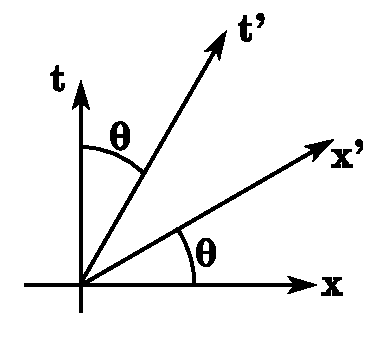
\includegraphics[width=5cm]{./figures/SROb_1.pdf}
\caption{洛伦兹变换的斜坐标表达,其中$\tan{\theta}=v/c$,两坐标轴的拉伸比例均为$(1+v^2/c^2)/(1-v^2/c^2)$.} \label{SROb_fig1}
\end{figure}




